\chapter{Ontologie}
In questo capitolo si andranno a mostrare le ontologie prese in esame: CarOnto, ControlOnto e MapOnto.

\section{Classi di CarOnto}
\index{Classi di CarOnto}

L'ontologia ``CarOnto" contiene diverse classi e sottoclassi che modellano un veicolo, quali:
\begin{itemize}
\item \textbf{\textit{CarParts}}, ovvero le parti del veicolo, composte dal motore (\textit{Engine}) e dai vari sensori (\textit{Sensor}) come \textit{Camera}, \textit{CAN}, \textit{GPS}, \textit{Lidar} e \textit{Sonar}.
\item \textbf{\textit{Trajectory}}, ovvero la traiettoria del veicolo, composte dal tracciato (\textit{Path}) e dai vari profili di velocit� (\textit{SpeedProfile}) come accelerazione (\textit{Acceleration}), velocit� costante (\textit{CostantSpeed}) e decelerazione (\textit{Deceleration}).
\item \textbf{\textit{Vehicle}}, ovvero dal tipo di veicolo. Questa ontologia suddivide i veicoli in tre categorie: 
	\begin{itemize}
	\item \textit{Automobile} nella quale sono presenti bus (\textit{Bus}), veicoli regolari (\textit{RegularVehicle}), veicoli speciali\footnote{Con veicoli speciali l'ontologia intende quei veicoli che non sono soggetti alle consuete regole di precedenza come filobus o tram.} (\textit{SpecialVehicle}) e truck (\textit{Truck}).
	\item \textit{Bicycle};
	\item \textit{Motorcycle};
	\end{itemize}
\end{itemize}
\begin{figure}[h]
    \centering
    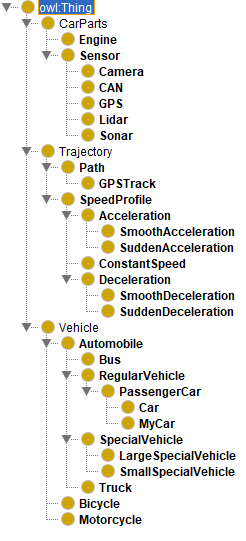
\includegraphics[width=0.40\textwidth]{img/car_class.png}
   	\caption{Classi di CarOnto}
	\label{fig:car_class}
\end{figure}

\newpage

\section{Classi di ControlOnto}
\index{Classi di ControlOnto}
L'ontologia ``ControlOnto" contiene diverse classi e sottoclassi che modellano i vari controlli che vengono effettuati da un veicolo ADAS, quali:
\begin{itemize}
	\item \textbf{\textit{DrivingAction}}, azioni effettuate dal veicolo come: partire (\textit{Go}), proseguire (\textit{GoForward}), far retromarcia (\textit{GoBackward}), fermarsi (\textit{Stop}) e cos� via;
	\item \textbf{\textit{LaneChange}}, modella il cambio di linea che pu� essere da destra (\textit{RightLaneChange}) o da sinistra (\textit{LeftLaneChange});
	\item \textbf{\textit{Path}}, ovvero il percorso che il veicolo deve seguire;
	\item \textbf{\textit{RoadCondition}}, la condizione della strada;
	\item \textbf{\textit{TrafficSignalControl}}, modella le azioni da effettuare di in presenza di un semaforo\footnote{Traffic lights e traffic signal sono sinonimi di inglese e corrispondono alla parola ``semaforo" in italiano.} come: procedere in presenza del verde (\textit{GreenGo}), fermasi in presenza del rosso (\textit{RedStop}) e giallo (\textit{Yellow});
	\item \textbf{\textit{Warning}}, modella i possibili avvisi tra cui: quello di collisione (\textit{CollisionWarning}), quello di deviazione dalla corsia (\textit{LaneDepartureWarning}) e quello di superamento dei limiti di velocit� (\textit{OverSpeedWarning}).
\end{itemize}
\begin{figure}[h]
    \centering
    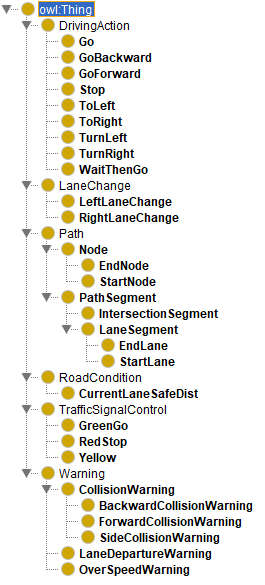
\includegraphics[width=0.40\textwidth]{img/control_class.png}
   	\caption{Classi di ControlOnto}
	\label{fig:control_class}
\end{figure}
\newpage

\section{Classi di MapOnto}
\index{Classi di MapOnto}
L'ontologia ``MapOnto" rappresenta la mappa stradale di un'area con segnaletica, quali:
\begin{itemize}
	\item \textbf{\textit{LivingThing}}, possibili esseri viventi presenti nell'area come un umano (\textit{Human});
	\item \textbf{\textit{Object}}, possibili oggetti presenti nell'area come un palo di utilit� (\textit{UtilityPole});
	\item \textbf{\textit{\textit{Place}}}, il luogo che pu� essere:
	\begin{itemize}
		\item un servizio (\textit{Amenity}) come ristorante, negozio e cos� via;
		\item un edificio (\textit{Building}) come ospedale, banca, ufficio postale, ecc.;
		\item un'infrastruttura (\textit{Infrastructure}) come aeroporto, stazione, distributore di benzina o un casello;
		\item un luogo naturale (\textit{NaturalPlace}) come un lago, un fiume o una foresta.
	\end{itemize}	  
	\item \textbf{\textit{RouteOfTransportation}}, la via di trasporto che contiene la parte e il tipo di strada (\textit{RoadPart} e \textit{RoadType}) e il limite di velocit� vigente (\textit{SpeedLimit});
	\item \textbf{\textit{Time}}, il momento della giornata:
	\begin{itemize}
		\item prima mattina (\textit{EarlyMorning});
		\item mattina (\textit{Morning});
		\item mezzogiorno (\textit{Noon});
		\item sera (\textit{Evening});
		\item mezzanotte (\textit{Midnight});
		\item notte (\textit{Night}).
	\end{itemize}
	\item \textbf{\textit{TrafficSign}}\footnote{``Traffic sign" � traducibile con ``segnaletica stradale", da non confondersi con ``traffic signal" che invece � ``semaforo".\cite{roadsignssignals}}, modella i vari segnali stradali presenti.
	\item \textbf{\textit{TrafficSignal}}, modella la presenza di un semaforo.
\end{itemize}
\begin{figure}[h]
    \centering
    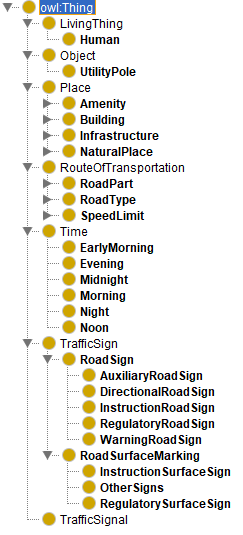
\includegraphics[width=0.40\textwidth]{img/map_class.png}
   	\caption{Classi di MapOnto}
	\label{fig:map_class}
\end{figure}
\newpage

\section{Propriet�}
\index{Propriet�}
Le propriet� servono a descrivere le caratteristiche di determinate classi, creando quindi una relazione con altre classi o con valori veri e propri.
Di seguito verranno mostrare le object property e le data property presenti nelle tre ontologie.
\begin{figure}[h]
\centering     %%% not \center
\subfigure[Object Property di CarOnto]{\label{fig:a}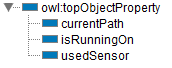
\includegraphics[width=60mm]{img/car_object_property.png}}
\subfigure[Data Property di CarOnto]{\label{fig:b}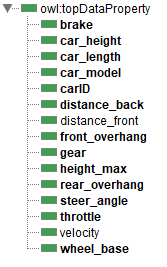
\includegraphics[width=60mm]{img/car_data_property.png}}
\caption{Object e data property di CarOnto}
\end{figure}

\begin{figure}[h]
\centering     %%% not \center
\subfigure[Object Property di ControlOnto]{\label{fig:a}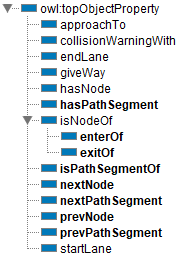
\includegraphics[width=60mm]{img/control_object_property.png}}
\subfigure[Data Property di ControlOnto]{\label{fig:b}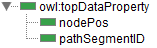
\includegraphics[width=60mm]{img/control_data_property.png}}
\caption{Object e data property di ControlOnto}
\end{figure}

\begin{figure}[h]
\centering     %%% not \center
\subfigure[Object Property di MapOnto]{\label{fig:a}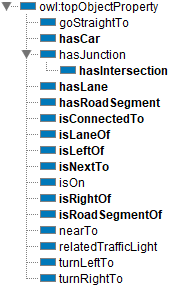
\includegraphics[width=60mm]{img/map_object_property.png}}
\subfigure[Data Property di MapOnto]{\label{fig:b}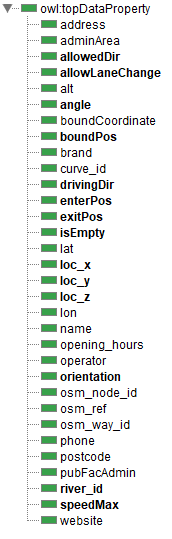
\includegraphics[width=60mm]{img/map_data_property.png}}
\caption{Object e data property di MapOnto}
\end{figure}



